%=============================================================================
%  Spread Builder — Mathematical Notes & Documentation
%  Study Notes + Technical Reference | Dark Wing Project
%=============================================================================
\documentclass[10pt,a4paper,twocolumn]{article}

%--- Geometry ----------------------------------------------------------------
\usepackage[a4paper,top=1.8cm,bottom=1.8cm,left=1.5cm,right=1.5cm,
            columnsep=0.7cm]{geometry}

%--- Math --------------------------------------------------------------------
\usepackage{amsmath,amssymb,amsthm,mathtools}

%--- Typography --------------------------------------------------------------
\usepackage[T1]{fontenc}
\usepackage{lmodern}
\usepackage{microtype}
\usepackage{parskip}
\setlength{\parskip}{2pt}

%--- Colours -----------------------------------------------------------------
\usepackage{xcolor}
\definecolor{codebg}{RGB}{245,247,250}
\definecolor{codeframe}{RGB}{180,195,220}
\definecolor{keyword}{RGB}{0,80,180}
\definecolor{comment}{RGB}{80,115,80}
\definecolor{string}{RGB}{160,40,20}
\definecolor{mathbluebg}{RGB}{230,240,255}
\definecolor{mathblue}{RGB}{10,60,160}
\definecolor{accent}{RGB}{25,95,195}
\definecolor{greenbg}{RGB}{230,250,232}
\definecolor{greenframe}{RGB}{50,155,70}
\definecolor{yellowbg}{RGB}{255,252,230}
\definecolor{yellowframe}{RGB}{180,150,0}
\definecolor{notebg}{RGB}{248,245,255}
\definecolor{noteframe}{RGB}{120,80,180}

%--- Code listings -----------------------------------------------------------
\usepackage{listings}
\lstdefinestyle{python}{
  language=Python,
  backgroundcolor=\color{codebg},
  frame=single,rulecolor=\color{codeframe},
  basicstyle=\ttfamily\fontsize{6.5}{8}\selectfont,
  keywordstyle=\bfseries\color{keyword},
  commentstyle=\itshape\color{comment},
  stringstyle=\color{string},
  numbers=left,numberstyle=\tiny\color{gray!70},
  numbersep=4pt,breaklines=true,tabsize=2,
  showstringspaces=false,aboveskip=3pt,belowskip=3pt,
  xleftmargin=12pt,
}
\lstdefinestyle{pythonplain}{
  language=Python,
  backgroundcolor=\color{codebg},
  frame=single,rulecolor=\color{codeframe},
  basicstyle=\ttfamily\fontsize{6.5}{8}\selectfont,
  keywordstyle=\bfseries\color{keyword},
  commentstyle=\itshape\color{comment},
  stringstyle=\color{string},
  numbers=none,breaklines=true,tabsize=2,
  showstringspaces=false,aboveskip=3pt,belowskip=3pt,
  xleftmargin=4pt,
}

%--- TikZ --------------------------------------------------------------------
\usepackage{tikz}
\usetikzlibrary{shapes.geometric,arrows.meta,positioning,calc,
                backgrounds,decorations.pathreplacing,fit}
\raggedbottom

\tikzset{
  fc_start/.style={rectangle,rounded corners=5pt,
    draw=accent,fill=accent!18,
    text width=4.4cm,align=center,
    font=\footnotesize\bfseries,
    inner sep=4pt,minimum height=0.6cm},
  fc_proc/.style={rectangle,
    draw=black!55,fill=white,
    text width=4.4cm,align=center,
    font=\footnotesize,
    inner sep=3pt,minimum height=0.58cm},
  fc_dec/.style={diamond,aspect=2.5,
    draw=accent,fill=accent!9,
    text width=2.9cm,align=center,
    font=\fontsize{6.2}{7.2}\selectfont,
    inner sep=1pt},
  fc_out/.style={rectangle,rounded corners=3pt,
    draw=greenframe,fill=greenbg,
    text width=4.4cm,align=center,
    font=\footnotesize,
    inner sep=3pt,minimum height=0.58cm},
  fc_side/.style={rectangle,
    draw=black!45,fill=yellow!10,
    text width=2.0cm,align=center,
    font=\fontsize{6.2}{7.2}\selectfont,
    inner sep=2pt,minimum height=0.52cm},
  arr/.style={-Stealth,semithick,draw=black!65},
}

%--- Boxes -------------------------------------------------------------------
\usepackage[most]{tcolorbox}
\tcbset{
  mathbox/.style={colback=mathbluebg,colframe=mathblue,
    fonttitle=\bfseries\small,title=#1,
    boxrule=0.5pt,top=3pt,bottom=3pt,left=4pt,right=4pt,
    before skip=4pt,after skip=4pt},
  exbox/.style={colback=yellowbg,colframe=yellowframe,
    fonttitle=\bfseries\small,title=#1,
    boxrule=0.5pt,top=3pt,bottom=3pt,left=4pt,right=4pt,
    before skip=4pt,after skip=4pt},
  resultbox/.style={colback=greenbg,colframe=greenframe,
    fonttitle=\bfseries\small,title=#1,
    boxrule=0.5pt,top=3pt,bottom=3pt,left=4pt,right=4pt,
    before skip=4pt,after skip=4pt},
  codebox/.style={colback=codebg,colframe=codeframe,
    fonttitle=\bfseries\small\color{accent},title=#1,
    boxrule=0.5pt,top=2pt,bottom=2pt,left=2pt,right=2pt,
    before skip=4pt,after skip=4pt},
  notebox/.style={colback=notebg,colframe=noteframe,
    fonttitle=\bfseries\small,title=#1,
    boxrule=0.5pt,top=3pt,bottom=3pt,left=4pt,right=4pt,
    before skip=4pt,after skip=4pt},
}

%--- Tables ------------------------------------------------------------------
\usepackage{booktabs,array,multirow}

%--- Header / Footer ---------------------------------------------------------
\usepackage{fancyhdr}
\usepackage[hidelinks]{hyperref}
\pagestyle{fancy}\fancyhf{}
\fancyhead[L]{\footnotesize\textbf{Spread Builder --- Study Notes}}
\fancyhead[R]{\footnotesize Project Dark-Wing}
\fancyfoot[C]{\footnotesize\thepage}
\renewcommand{\headrulewidth}{0.4pt}

%--- Floats / Captions -------------------------------------------------------
\usepackage{float,caption,graphicx}
\captionsetup{font=scriptsize,labelfont=bf,skip=3pt}

%--- Section formatting ------------------------------------------------------
\usepackage{titlesec}
\titlespacing*{\section}{0pt}{7pt}{3pt}
\titlespacing*{\subsection}{0pt}{5pt}{2pt}
\titlespacing*{\subsubsection}{0pt}{3pt}{1pt}
\titleformat{\section}{\normalfont\bfseries\color{accent}}{}{0em}{}
  [{\color{accent}\titlerule[0.5pt]}]
\titleformat{\subsection}{\normalfont\bfseries\small}{}{0em}{}
\titleformat{\subsubsection}{\normalfont\itshape\small}{}{0em}{}

%=============================================================================
\begin{document}
%=============================================================================

\twocolumn[{%
\begin{center}
  {\LARGE\bfseries\color{accent}
    Spread Construction in Pairs Trading}\\[5pt]
  {\large\bfseries \texttt{spread\_builder.py} --- Mathematical Notes \& Documentation}\\[3pt]
  {\small\itshape Cointegration-Based Spread, OLS Hedge Ratio, and Kalman Filter Interface}\\[3pt]
  {\small Project Dark-Wing \quad|\quad \today}
\end{center}
\vspace{4pt}
\noindent\rule{\linewidth}{0.5pt}\vspace{2pt}
\begin{quote}\small
\textbf{Abstract.}~Once two or more assets are confirmed cointegrated, their
\emph{spread} is the stationary linear combination that oscillates around a
fixed mean.  This document derives three spread constructions used in the
\texttt{SpreadBuilder} class: OLS-estimated spread (Engle-Granger style),
fixed-beta spread (from Johansen or Kalman), and the Johansen ECT spread.
The key output, a stationary $S_t$ series, feeds directly into the
\texttt{HalfLife}, \texttt{ZScore}, and \texttt{Kalman\_Filter} modules.
\end{quote}
\noindent\rule{\linewidth}{0.5pt}\vspace{5pt}
}]

%=============================================================================
\section{Why Do We Build a Spread?}
%=============================================================================

After the Johansen test (Step 3) confirms cointegration rank $r^*\geq1$,
we know a stationary linear combination $S_t = \boldsymbol\beta'\mathbf{X}_t$
exists.  This spread is the \emph{mean-reverting signal} we trade.

\begin{tcolorbox}[notebox={Key Intuition}]
If two stocks move together in the long run, their price difference
will deviate from equilibrium occasionally but always return.
This deviation \emph{is} the spread $S_t$, and trading it is
\emph{statistically arbitrage}.
\end{tcolorbox}

\noindent\textbf{Three modes} are supported:
\begin{itemize}\setlength\itemsep{1pt}
  \item \textbf{OLS}: Estimate $\beta$ from data (2-asset).
  \item \textbf{Fixed-beta}: Supply $\beta$ from Johansen/Kalman.
  \item \textbf{Johansen ECT}: Multi-asset matrix spread.
\end{itemize}

%=============================================================================
\section{Mode 1: OLS Spread (2-Asset)}
%=============================================================================

\subsection{The Cointegrating Regression}

For two log-price series $Y_t$ and $X_t$, the cointegrating regression is:
\begin{tcolorbox}[mathbox={Formula 1 --- Cointegrating Regression}]
\vspace{-4pt}
\begin{equation}\label{eq:coint_reg}
  Y_t = \alpha + \beta\,X_t + \varepsilon_t
\end{equation}
\vspace{-3pt}
If $Y_t$ and $X_t$ are cointegrated, then $\varepsilon_t = S_t$ is I(0)
(stationary).  $\beta$ is the \emph{hedge ratio}.
\end{tcolorbox}

\subsection{OLS Estimation of Hedge Ratio}

We minimise the sum of squared residuals:
\begin{tcolorbox}[mathbox={Formula 2 --- OLS in Matrix Form}]
\vspace{-4pt}
\begin{equation}
  \hat{\boldsymbol\theta} =
    \begin{bmatrix}\hat\alpha\\\hat\beta\end{bmatrix}
    = (\mathbf{X}^\top\mathbf{X})^{-1}\mathbf{X}^\top\mathbf{y}
\end{equation}
where $\mathbf{X} = [\mathbf{1},\, X_t]$ (design matrix),\;
$\mathbf{y} = Y_t$ (response).
\vspace{-2pt}
\end{tcolorbox}

\subsection{Spread Construction}

Once $\hat\alpha$ and $\hat\beta$ are estimated:
\begin{tcolorbox}[mathbox={Formula 3 --- OLS Spread}]
\vspace{-4pt}
\begin{equation}\label{eq:ols_spread}
  S_t = Y_t - \hat\alpha - \hat\beta\, X_t
\end{equation}
\vspace{-2pt}
$S_t$ should be I(0): verified by ADF/KPSS in \texttt{VECMDiagnostics}.
\end{tcolorbox}

\noindent\textbf{Financial meaning.}~
$\hat\beta$ tells us how many units of $X$ to hold short for each unit of
$Y$ held long.  This is the \emph{dollar-neutral} hedge ratio.  A $\beta > 1$
means $X$ is the more expensive leg; we hold less of it per unit of $Y$.

%=============================================================================
\section{Mode 2: Fixed-Beta Spread}
%=============================================================================

When $\beta$ is supplied externally (e.g.\ Johansen's $\boldsymbol\beta$
or a Kalman-filtered $\hat\beta_t$), we skip OLS:

\begin{tcolorbox}[mathbox={Formula 4 --- Fixed-Beta Spread}]
\vspace{-4pt}
\begin{equation}\label{eq:fixed_spread}
  S_t = Y_t - \beta\, X_t, \quad \alpha = 0
\end{equation}
\vspace{-2pt}
No intercept is removed.  This is appropriate when the cointegrating
vector already encodes the long-run mean.
\end{tcolorbox}

\noindent\textbf{When to use.}~
Use \texttt{mode='fixed\_beta'} when you have a Johansen-estimated $\beta$
from \texttt{johansen.py}, or when the Kalman filter is actively updating
$\beta_t$ at each timestep.

%=============================================================================
\section{Mode 3: Johansen ECT (Multi-Asset)}
%=============================================================================

\subsection{The ECT from Johansen}

For $m$ assets with cointegrating rank $r^*$, Johansen provides the
$(m \times r^*)$ cointegrating matrix $\boldsymbol\beta$.  Each column is
a cointegrating vector.

\begin{tcolorbox}[mathbox={Formula 5 --- Johansen ECT Spread}]
\vspace{-4pt}
\begin{equation}\label{eq:ect}
  \mathbf{S}_t = \boldsymbol\beta'\,\mathbf{X}_t
  \quad\text{shape: } (r^* \times 1)
\end{equation}
\vspace{-2pt}
Each row $S_{j,t} = \boldsymbol\beta_j'\mathbf{X}_t$ is a separate
cointegrating spread (ECT).  All $r^*$ ECT columns are stationary.
\end{tcolorbox}

In matrix form for all $T$ observations:
\[
  \underbrace{\mathbf{S}}_{T \times r^*}
  = \underbrace{\mathbf{X}}_{T \times m}\;
    \underbrace{\boldsymbol\beta}_{m \times r^*}
\]

\noindent\textbf{Financial meaning.}~
Each ECT column is a portfolio of all $m$ assets with weights given by the
corresponding column of $\boldsymbol\beta$.  Portfolio $j$ is orthogonal
to the unit-root component of $\mathbf{X}_t$, so it is stationary.

%=============================================================================
\section{Hedge Ratio Summary Table}
%=============================================================================

\begin{center}
{\small
\begin{tabular}{@{}p{1.7cm}p{2.0cm}p{2.0cm}@{}}
\toprule
Mode & $\beta$ source & Intercept?\\
\midrule
OLS & Estimated from data & Yes ($\hat\alpha$)\\
fixed\_beta & Supplied (Johansen/Kalman) & No\\
johansen\_ect & Johansen $\boldsymbol\beta$ matrix & No\\
\bottomrule
\end{tabular}
}
\end{center}

%=============================================================================
\section{Kalman Filter Interface Contract}
%=============================================================================

The \texttt{Kalman\_Filter/} module requires three aligned series:

\begin{tcolorbox}[notebox={Interface: SpreadBuilder $\to$ Kalman}]
\begin{itemize}\setlength\itemsep{1pt}
  \item \texttt{spread\_series()} $\to$ $S_t$ — observation for filter.
  \item \texttt{y\_series()} $\to$ $Y_t$ — dependent leg.
  \item \texttt{x\_series()} $\to$ $X_t$ — independent leg.
\end{itemize}
All three share the same \texttt{DatetimeIndex}.
In \texttt{complete\_kalman\_filter.py}:\\
\texttt{correction(y=Y\_t, x=X\_t)} produces the Kalman spread
$s_t = Y_t - \hat\beta_t \cdot X_t$.
\end{tcolorbox}

%=============================================================================
\section{Code Flowchart --- \texttt{SpreadBuilder}}
%=============================================================================

\begin{figure}[H]
\centering
\resizebox{\columnwidth}{!}{%
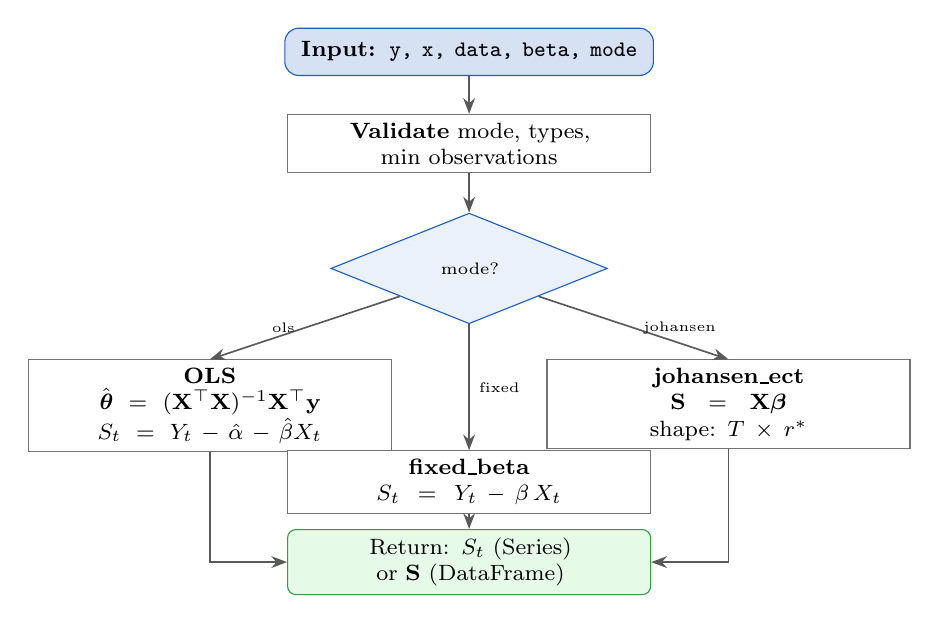
\begin{tikzpicture}[node distance=0.48cm,
                    every node/.style={font=\scriptsize}]
  \node (in) [fc_start]
    {Input: \texttt{y, x, data, beta, mode}};
  \node (val) [fc_proc, below=of in]
    {\textbf{Validate} mode, types,\\ min observations};
  \node (d1) [fc_dec, below=0.5cm of val]
    {mode?};
  % OLS branch
  \node (ols) [fc_proc, below left=0.8cm and 0.1cm of d1]
    {\textbf{OLS}\\
     $\hat{\boldsymbol\theta}=(\mathbf{X}^\top\mathbf{X})^{-1}\mathbf{X}^\top\mathbf{y}$\\
     $S_t = Y_t-\hat\alpha-\hat\beta X_t$};
  % fixed beta branch
  \node (fb) [fc_proc, below=1.6cm of d1]
    {\textbf{fixed\_beta}\\
     $S_t = Y_t - \beta\,X_t$};
  % johansen_ect branch
  \node (jct) [fc_proc, below right=0.8cm and 0.1cm of d1]
    {\textbf{johansen\_ect}\\
     $\mathbf{S} = \mathbf{X}\boldsymbol\beta$\\
     shape: $T\times r^*$};
  \node (out) [fc_out, below=2.6cm of d1]
    {Return: $S_t$ (Series)\\ or $\mathbf{S}$ (DataFrame)};

  \draw[arr] (in) -- (val);
  \draw[arr] (val) -- (d1);
  \draw[arr] (d1.south west) -- node[left,font=\tiny]{ols} (ols.north);
  \draw[arr] (d1.south)      -- node[right,font=\tiny]{fixed} (fb.north);
  \draw[arr] (d1.south east) -- node[right,font=\tiny]{johansen} (jct.north);
  \draw[arr] (ols.south)  |- (out.west);
  \draw[arr] (fb.south)   -- (out.north);
  \draw[arr] (jct.south)  |- (out.east);
\end{tikzpicture}
}
\caption{Execution flowchart for \texttt{SpreadBuilder.build()}.}
\label{fig:spread_flow}
\end{figure}

%=============================================================================
\section{Worked Example}
%=============================================================================

\begin{tcolorbox}[exbox={Setup}]
Log-prices: $Y = [2.30, 2.64, 2.08, 2.77, 2.49]$,\;
$X = [3.00, 3.40, 2.90, 3.50, 3.20]$.\\
Mode: \textbf{OLS}, include intercept.
\end{tcolorbox}

\noindent\textbf{Step 1 --- Design matrix:}
\[
  \mathbf{X} = \begin{bmatrix}
    1 & 3.00\\ 1 & 3.40\\ 1 & 2.90\\ 1 & 3.50\\ 1 & 3.20
  \end{bmatrix},\quad
  \mathbf{y} = \begin{bmatrix}2.30\\2.64\\2.08\\2.77\\2.49\end{bmatrix}
\]

\noindent\textbf{Step 2 --- OLS estimate:}
\[
  \hat{\boldsymbol\theta} \approx \begin{bmatrix}-0.12\\0.79\end{bmatrix}
  \;\Rightarrow\; \hat\alpha=-0.12,\;\hat\beta=0.79
\]

\noindent\textbf{Step 3 --- Spread:}
\begin{align*}
  S_1 &= 2.30 - (-0.12) - 0.79\times3.00 = +0.05\\
  S_2 &= 2.64 - (-0.12) - 0.79\times3.40 = +0.07\\
  &\vdots
\end{align*}

\begin{tcolorbox}[resultbox={Interpretation}]
$\hat\beta = 0.79$: for every 1 unit of $Y$ long, we short $0.79$ units
of $X$.  The spread $S_t \approx 0$ with small deviations --- confirming
cointegration.  The intercept $\hat\alpha=-0.12$ absorbs the long-run
level difference.
\end{tcolorbox}

%=============================================================================
\section{Python Implementation Snippets}
%=============================================================================

\begin{tcolorbox}[codebox={OLS beta estimation}]
\begin{lstlisting}[style=pythonplain]
def _ols_beta(self) -> tuple:
    y = self._y.values
    x = self._x.values
    if self.include_intercept:
        X = np.column_stack([np.ones(len(x)), x])
        coef = np.linalg.lstsq(X, y, rcond=None)[0]
        alpha, beta = float(coef[0]), float(coef[1])
    else:
        coef = np.linalg.lstsq(
            x.reshape(-1,1), y, rcond=None)[0]
        alpha, beta = 0.0, float(coef[0])
    return alpha, beta
\end{lstlisting}
\end{tcolorbox}

\begin{tcolorbox}[codebox={Johansen ECT construction}]
\begin{lstlisting}[style=pythonplain]
# mode = 'johansen_ect'
ect_vals = self._data.values @ self._beta_input
# shape: (T, r*)
self._ect_df = pd.DataFrame(
    ect_vals, index=self._data.index,
    columns=[f"ECT_{j+1}" for j in range(r)])
# primary spread = first ECT column
self._spread = self._ect_df["ECT_1"].rename("spread")
\end{lstlisting}
\end{tcolorbox}

%=============================================================================
\section{Pipeline Position}
%=============================================================================

\begin{center}
{\small
\begin{tabular}{@{}clp{2.0cm}@{}}
\toprule
Step & Module & Output\\
\midrule
1 & \texttt{TS\_stationarity\_test} & I(1) confirmation\\
2 & \texttt{VAR lag select} & $k^*$ lags\\
3 & \texttt{johansen.py} & $r^*$, $\boldsymbol\beta$\\
4 & \texttt{fit\_vecm.py} & $\alpha$, $\boldsymbol\beta$, ECT\\
4.5 & \texttt{diagnostics.py} & Health score gate\\
\textbf{5a} & \textbf{\texttt{spread\_builder.py}} & $S_t$ series\\
5b & \texttt{half\_life.py} & $\tau$, $\kappa$\\
5c & \texttt{zscore.py} & $Z_t$, signals\\
6 & \texttt{Kalman\_Filter/} & Dynamic $\hat\beta_t$\\
\bottomrule
\end{tabular}
}
\end{center}

\end{document}
